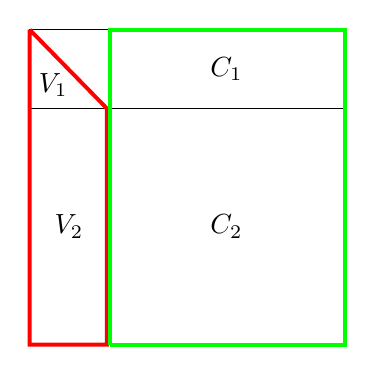
\begin{tikzpicture}
\draw[semithick] (0,0) -- (4,0) -- (4,4)-- (0,4)-- (0,0);

\draw[semithick] (1,0) -- (1,4);
\draw[semithick] (0,3) -- (4,3);
\draw[red, line width=0.5mm, opacity=1] (0,4) -- (0,0) -- (0.98,0) -- (0.98,3) -- (0,4);
\draw[green, line width=0.5mm, opacity=1] (1.02,0) -- (4,0) -- (4,4)-- (1.02,4)-- (1.02,0);


%\draw[decorate, decoration={brace,mirror}, yshift=-.5ex]  (0,0) -- node[below=0.4ex] {$k$}  (.95,0);
%\draw[decorate, decoration={brace}, xshift=-.5ex]  (0,3) -- node[left=0.2ex] {$k$}  (0,4);
%\draw[decorate, decoration={brace,mirror}, yshift=-.5ex]  (1.05,0) -- node[below=0.4ex] {$n$}  (4,0);
%\draw[decorate, decoration={brace}, xshift=-3ex]  (0,0) -- node[left=0.4ex] {$m$}  (0,4);

\draw (0.3,3.3) node {$V_1$};
\draw (0.5,1.5) node {$V_2$};
\draw (2.5,3.5) node {$C_1$};
\draw (2.5,1.5) node {$C_2$};

\end{tikzpicture}